% Metodologia.
%

%   - Quina és l'arquitectura/enfocament general de la solució?
%   - Quines decisions de disseny s'han pres i per què (alternatives descartades i motiu)?
%   - Quina metodologia de treball s'ha seguit (iteratiu, experimental, disseny d'experiments, mètrica d'avaluació prevista...)?
%
% Si el teu treball és de desenvolupament de software, comença amb una secció breu de requisits (funcionals i no funcionals).

Aquest capítol descriu el disseny experimental dissenyat per avaluar i quantificar l'impacte sobre el rendiment de Kubernetes (K3s) en comparació amb una arquitectura nativa basada en Systemd. L'estudi s'articula mitjançant una comparativa A/B automatitzada per garantir la reproductibilitat de totes les proves.

\section{Especificacions de l'Entorn Experimental (Testbed)}
Per contextualitzar adequadament l'avaluació en maquinari de capacitats reduïdes i assegurar la replicabilitat de l'experiment, la Taula~\ref{tab:testbed_general} recull les característiques tècniques de la plataforma de proves virtualitzada.

\begin{table}[htbp]
    \centering
    \begin{tabular}{l p{10.5cm}}
        \hline
        \textbf{Component / Paràmetre} & \textbf{Especificació tècnica} \\ \hline
        Arquitectura base (amfitrió) & Intel Core i9-14900HX (x86\_64) \\
        Entorns de virtualització & WSL2 (Node Mestre) / VMware Workstation Player 17 (Nodes \textit{Workers}) \\
        S.O. i nucli (Mestre) & Ubuntu 22.04.5 LTS -- Linux Kernel 6.18.x (Microsoft Standard) \\
        S.O. i nucli (\textit{Workers}) & Ubuntu 24.04.4 LTS (mode \textit{headless}) -- Linux Kernel 6.8.0-138-generic \\
        Recursos Node Mestre & 32 vCPUs, 16~GB RAM, 1~TB d'emmagatzematge \\
        Recursos \textit{Workers} (Systemd) & 2 vCPUs, 2~GB RAM, 20~GB d'emmagatzematge NVMe/SATA \\
        Recursos \textit{Workers} (K3s) & 2 vCPUs, 4~GB RAM, 35~GB d'emmagatzematge (ampliat per prevenir fallades per \textit{Out-Of-Memory}) \\
        Versions de programari & Podman (v4.9.3), Systemd (v255), K3s (v1.35.4+k3s1), Ansible (v2.17.14), Go (v1.25.9) \\
        Xarxa i connectivitat & Gestió via \textit{Netplan} (DHCP), interfície \texttt{ens33}, CNI Flannel (\texttt{10.42.1.0/24}) \\ \hline
    \end{tabular}
    \caption{Característiques generals de l'entorn experimental.}
    \label{tab:testbed_general}
\end{table}

A causa de la petjada de memòria estructural associada al pla de control de Kubernetes, es van establir dues configuracions de maquinari en funció de l'arquitectura avaluada:

\begin{itemize}
    \item \textbf{Fase nativa (Systemd + Podman):} Els nodes perimetrals es van configurar amb un perfil ajustat per emular un dispositiu \textit{Edge} restrictiu: \textbf{2 vCPUs}, \textbf{2~GB de RAM} i un volum d'emmagatzematge de \textbf{20~GB}. Aquest dimensionament permet avaluar l'operativitat de la pila nativa en condicions de recursos mínims.
    \item \textbf{Fase distribuïda (K3s):} Per a l'entorn amb K3s, va caldre ampliar els recursos assignats a la màquina virtual fins a \textbf{4~GB de RAM} i \textbf{35~GB} de disc. Aquesta adaptació respon a un requisit pràctic: amb només 2~GB de memòria, la concurrència del pla de control i el connector de xarxa (Flannel) exhauria el marge disponible abans d'iniciar l'execució del model d'Intel·ligència Artificial, provocant aturades prematures per exhauriment de memòria (\textit{Out-Of-Memory}).
\end{itemize}

\section{Disseny Iteratiu i Selecció de Protocols}
L'estudi es va estructurar en quatre etapes iteratives amb l'objectiu d'identificar prèviament la configuració de xarxa més eficient i impedir que la capa de comunicació actués com a coll d'ampolla durant l'avaluació comparativa:

\begin{itemize}
    \item \textbf{Fase 1: Exploració inicial de protocols en entorn natiu:} Es va mesurar l'impacte dels protocols de transport (HTTP, gRPC, ZeroMQ) i dels formats de codificació (text pla enfront de binari) sobre la pila base de Systemd utilitzant la càrrega de treball MNIST. L'anàlisi de paràmetres com el temps de resposta, la taxa d'èxit i el consum de recursos va confirmar que la combinació de ZeroMQ amb formats binaris oferia el rendiment més sòlid.
    \item \textbf{Fase 2: Avaluació de la serialització binària (Protobuf enfront de MessagePack):} Dins de les opcions binàries, es va dur a terme una comparativa a quatre bandes: HTTP-JSON, gRPC-Protobuf, ZeroMQ-Protobuf i ZeroMQ-MessagePack. Tot i les propietats de Protobuf en entorns estructurats, MessagePack va resultar més adient a causa de les característiques del conjunt MNIST:
    \begin{itemize}
        \item \textit{Sobrecàrrega en Protobuf:} Definir la matriu de la imatge mitjançant el camp \texttt{repeated int32} en el fitxer \texttt{.proto} incrementa la mida del missatge de 784 bytes a més de 2~KB, provocant un consum excessiu de CPU durant els cicles de codificació i descodificació píxel a píxel. Encara que recórrer al tipus \texttt{bytes} esmorteïa aquesta penalització, eliminava l'avantatge del tipat estricte propi de la solució.
        \item \textit{Eficiència en MessagePack:} Aquest mecanisme permet empaquetar directament el flux binari sense processament intermedi (\textit{bin type}) a partir de les estructures de memòria, minimitzant l'ús de processador i mantenint una transmissió compacta.
    \end{itemize}
    \item \textbf{Fase 3: Validació del protocol sobre l'orquestrador:} El comportament observat amb ZeroMQ i MessagePack es va reproduir sobre el clúster de Kubernetes, verificant que el patró d'eficiència es mantenia constant independentment de la plataforma subjacent. Com a distribució distribuïda, es va optar per K3s pel seu disseny orientat específicament a plataformes \textit{Edge}.
    \item \textbf{Fase 4: Comparativa arquitectònica final:} Amb el canal de comunicació fixat en ZeroMQ-MessagePack per descartar limitacions de xarxa, es van executar les proves d'estrès definitives per contraposar directament l'arquitectura nativa (Systemd) amb la solució distribuïda (K3s).
\end{itemize}

\section{Selecció del Model d'IA}
Perquè la càrrega fos representativa d'un cas d'ús real de visió artificial, es va descartar l'ús d'un Perceptró Multicapa (MLP) simple en favor d'una Xarxa Neuronal Convolucional (CNN). Aquest tipus de xarxa aprofita la correlació espacial dels píxels mitjançant operacions matricials intensives en capes convolucionals i denses. Els tensors generats sotmeten el processador i la memòria a un volum d'inferència continu, permetent avaluar el rendiment d'ambdues solucions sota una càrrega computacional representativa.
\begin{figure}[H]
    \centering
    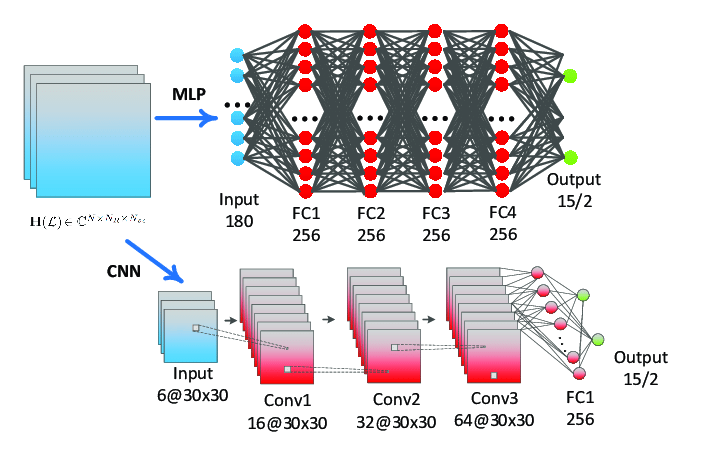
\includegraphics[width=0.85\textwidth]{sources/mlp_cnn_architecture.png}
    \caption{Arquitectura comparativa de xarxes MLP i CNN dissenyades per a tasques de classificació i regressió. Font: Adaptada de \cite{xiang2019robust}.}
    \label{fig:arquitectura_mlp_cnn}
\end{figure}

\section{Topologia i Estratègia de Desplegament (Patró \textit{Air-Gapped})}
L'arquitectura de la prova separa el node de gestió dels nodes d'execució (\textit{Workers}). Amb la intenció d'aïllar els resultats de variacions derivades de la connectivitat externa o del trànsit d'Internet, es va seguir una metodologia \textit{Air-Gapped}:

\begin{itemize}
    \item \textbf{Construcció centralitzada:} La generació i compilació dels binaris i imatges es centralitza al node mestre per no penalitzar la capacitat de càlcul dels nodes perimetrals.
    \item \textbf{Distribució local:} Els artefactes resultants es transfereixen directament a l'emmagatzematge intern de cada \textit{worker} abans d'iniciar les mesures.
    \item \textbf{Separació de responsabilitats:} Tant en Systemd com en K3s, l'execució de les tasques d'inferència queda confinada als nodes perimetrals, assegurant que el pla de gestió no interfereixi en els mesuraments de rendiment.
\end{itemize}

\section{Automatització i Reproduïbilitat (\textit{Pipeline} d'execució)}
La recollida de dades s'ha articulat mitjançant un flux de treball completament automatitzat per evitar desviacions manuals. Cada iteració segueix la seqüència següent:

\begin{itemize}
    \item \textbf{Purga i desplegament inicial:} S'esborren els contenidors i volums previs i s'elimina la memòria cau per reiniciar l'entorn des d'un estat base homogeni abans de cada cicle.
    \item \textbf{Període d'estabilització:} S'apliquen intervals d'espera programats per evitar fenòmens d'estrangulament tèrmic (\textit{thermal throttling}) al maquinari i permetre que els serveis base assoleixin un estat estacionari abans de mesurar els consums.
    \item \textbf{Cicle de càrrega:} S'aplica un patró de sol·licituds concurrents continuat per avaluar el comportament del sistema sota condicions de pressió operativa sostinguda.
    \item \textbf{Centralització de registres:} Les lectures generades s'extreuen dels registres del sistema operatiu i s'emmagatzemen automàticament en un fitxer estructurat de tipus CSV per facilitar el tractament estadístic posterior.
\end{itemize}

\section{Tècniques de Mesura i Mètriques d'Avaluació}
\label{subsec:metriques_avaluacio}
L'impacte de cada arquitectura es quantifica a través de quatre indicadors principals d'infraestructura i disponibilitat:

\begin{itemize}
    \item \textbf{Temps de Desplegament ($T_{deploy}$):} Interval temporal (expressat en segons) requerit per aprovisionar el node, establir les configuracions de servei i deixar les imatges a punt per a la inferència.
    \item \textbf{Consum de CPU en Repòs (\texttt{CPU\_Repòs}):} Percentatge mitjà d'ús de CPU atribuïble als dimonis de fons de la plataforma (\textit{kubelet}, \textit{containerd} o processos del sistema) en absència de trànsit de xarxa.
    \item \textbf{Consum de Memòria en Repòs (\texttt{RAM\_Repòs}):} Ocupació de memòria RAM associada estrictament a la pila de programari en estat d'espera, mesurada en megabytes (MB).
    \item \textbf{Temps Mitjà de Recuperació (MTTR):} Temps requerit pel sistema (en mil·lisegons) per restablir el servei després de provocar la terminació forçada del procés principal mitjançant senyals de caiguda abrupta.
\end{itemize}

\subsection{Tractament de Valors Atípics (Outliers)}
\label{subsec:tractament_dades}
Durant els assajos de tolerància a fallades sobre Kubernetes, es va registrar un valor anòmal en una de les iteracions, amb un temps de recuperació de 261.450~ms (\textasciitilde 4,3~minuts). Aquest retard va ser causat per una retenció temporal (\textit{lock}) en l'alliberament de la xarxa virtual gestionada per Flannel.

En comptes de suprimir la dada o recórrer a la imputació estadística, s'ha optat per segregar aquest registre de l'anàlisi de tendència central. Així, les mètriques resum (mitjana, mediana i desviació estàndard) es presenten excloent aquest valor per caracteritzar el comportament nominal de l'orquestrador en condicions d'estabilitat. No obstant això, el cas s'analitza de manera monogràfica en el capítol de resultats, ja que posa de manifest una vulnerabilitat pròpia dels mecanismes de coordinació en xarxes virtuals definides per programari (SDN).